\documentclass[xcolor=dvipsnames]{beamer}
%%%%%%%%%%%%%%%%%%%%%%%%%%%%%%%%%%%%
%
% Packages
%
%%%%%%%%%%%%%%%%%%%%%%%%%%%%%%%%%%%%
\usepackage{hyperref}
\usepackage{caption}
\usepackage{subcaption}
\usepackage{amsmath,amsfonts,amssymb}
\usepackage{lmodern}
\usepackage{graphicx}
\usepackage{caption}
\setcounter{MaxMatrixCols}{14}
\usepackage{multicol}
\usepackage{etoolbox}
\usepackage{bibentry}
\usepackage{dsfont}

\usepackage[utf8]{inputenc}
\usepackage[T1]{fontenc}
\usepackage[french]{babel}

\usepackage{babel,blindtext}
\usepackage{color}
\DeclareMathOperator*{\argmin}{arg\,min}
\usepackage{tikz}
\usetikzlibrary{shapes,shadows,arrows}

\setbeamercovered{dynamic}
\useinnertheme{rectangles}


%%%%%%%%%%%%%%%%%%%%%%%%%%%%%%%%%%%%
%
% Theme
%
%%%%%%%%%%%%%%%%%%%%%%%%%%%%%%%%%%%%
\usetheme{Boadilla}
\usecolortheme[named=Brown]{structure}
\usetheme[height=7mm]{Rochester}

\title{Formation de coalitions de "Prosumers" dans un environnement Smart Grid}
\author[N. Gensollen]{\textbf{Nicolas Gensollen}, Vincent Gauthier, Monique Becker, Micher Marot}
\institute[TSP]{
  CNRS SAMOVAR, Telecom SudParis\\
  Institut Mines\-Telecom\\[1ex]
  \texttt{nicolas.gensollen@telecom-sudparis.eu}
}
\date{10 Avril 2015}

%%%%%%%%%%%%%%%%%%%%%%%%%%%%%%%%%%%%
%
% Main Document
%
%%%%%%%%%%%%%%%%%%%%%%%%%%%%%%%%%%%%
\begin{document}



%%%%%%%%%%%%%%%%%%%%%%%%%%%%%%%%%%%%
%
% Slides 3
%
%%%%%%%%%%%%%%%%%%%%%%%%%%%%%%%%%%%%
\begin{frame}
	\frametitle{Sujet de thèse}

\begin{itemize}
	\item \textbf{Sujet :} \textit{Modeling and optimizing a distributed power network: A complex system approach of the 'prosumer' management in the smart grid}
	\item \textbf{Axe 1} : Etude de la formation de coalitions de prosumers
	\item Publications :
	\begin{itemize}
		\item \textit{Coalition Formation Algorithm of Prosumers in a Smart Grid Environment}, IEEE ICC 2015
		\item \textit{Stability and Performance of Coalitions of Prosumers Through Diversification in the Smart Grid}, Transactions on Smart Grid (en cours de révision)
	\end{itemize}
	\item \textbf{Axe 2} : Etude du controle d'un réseau électrique de prosumers
	\item Publications :
	\begin{itemize}
		\item \textit{Control of Prosumer Networks}, finalisation d'écriture
	\end{itemize}
\end{itemize}

\end{frame}


%%%%%%%%%%%%%%%%%%%%%%%%%%%%%%%%%%%%
%
% Slides 3
%
%%%%%%%%%%%%%%%%%%%%%%%%%%%%%%%%%%%%
\begin{frame}
	\frametitle{Axe 1, Prosumers et intérêt des coalitions}


\begin{itemize}
	\item \textbf{Prosumer} = Agent consommant et produisant de l'électricité
	\item Son objectif = optimiser ses bénéfices/dépenses et son utilisation de l'électricité
\end{itemize}
Pourquoi former des coalitions ?
\begin{itemize}
	\item DER = \textit{Distributed Energy Resources}	
	\item \textbf{Stabiliser} les DER basés sur des énergies intermittentes 
	\item \textbf{Décentraliser} la production
	\item \textbf{Rapprocher} la production de la consommation
	\item Permettre aux prosumers de \textbf{participer} en s'agrégeant
	\item Améliorer la \textbf{visibilité} des DER
\end{itemize}

\end{frame}


%%%%%%%%%%%%%%%%%%%%%%%%%%%%%%%%%%%%
%
% Slides 3
%
%%%%%%%%%%%%%%%%%%%%%%%%%%%%%%%%%%%%
\begin{frame}
	\frametitle{Objectifs de l'étude}
	
Objectifs :
\begin{itemize}
\item Construire un \textbf{modèle réaliste} de prosumer basé sur des données réelles
\item \textbf{Simuler} le comportement de ces prosumers sur une période donnée
\item Autoriser les prosumers à \textbf{vendre leur surplus} de production à l'opérateur de réseau
\item \textbf{Restreindre} l'accès au marché à des entités suffisamment \textbf{productrices} et \textbf{stables}
\item \textbf{Définir} une notion statistique de la \textbf{stabilité} d'une coalition
\item Élaborer un \textbf{processus de formation} de coalitions de prosumers stables
\item Montrer l'efficacité de ce processus
\end{itemize}

\end{frame}



%%%%%%%%%%%%%%%%%%%%%%%%%%%%%%%%%%%%
%
% Slides 3
%
%%%%%%%%%%%%%%%%%%%%%%%%%%%%%%%%%%%%
\begin{frame}
	\frametitle{Modèlisation des prosumers}

\begin{columns}
	\begin{column}{.5\textwidth}
		\begin{footnotesize}
			\begin{itemize}
				\item \textbf{But} : Obtenir un large spectre de profils de consommation / production
				\item Utilisation de \textbf{données météorologiques} (Vitesse du vent, Ensoleillement, Température)
				\item \textbf{Discrétisation} de l'espace autour des stations 
				\item Prosumers disposés aléatoirement 
				\item Pour tout agent i, on note $ P_{i}(t) $ la \textbf{production instantanée} (en W) disponible à l'instant t
				\item $ P_{i}(t) $ est la différence entre la production absolue de i et sa consommation
				\item Les traces $ P_{i}(t) $ sont obtenues par simulation
			\end{itemize}
		\end{footnotesize}
	\end{column}
	\begin{column}{.5\textwidth}
		\begin{figure}
			\includegraphics[width=6.1cm]{fig2.pdf}
		\end{figure}
	\end{column}
\end{columns}

\end{frame}

%%%%%%%%%%%%%%%%%%%%%%%%%%%%%%%%%%%%
%
% Slides 3
%
%%%%%%%%%%%%%%%%%%%%%%%%%%%%%%%%%%%%
\begin{frame}
	\frametitle{Contrats de production}
	
\begin{scriptsize}
\begin{itemize}
	\item Les coalitions sont formées pour le "jour J+1"
	\item Pour entrer sur le marché, une entité $ S $ doit estimer et annoncer une valeur de contrat $ P_{S}^{CRCT} $
	\item Volatilité de la production et de la consommation
	\item Un algorithme interne à la coalition doit maintenir $ P_{S}(t) = P_{S}^{CRCT}\ \forall t $ (batteries, charges différées, générateurs de backup...)
	\item Moins S dévie de $ P_{S}^{CRCT} $, plus le maintien de S est aisé et peu couteux 
	\item Parallèlement, plus $ P_{S}^{CRCT} $ est élevé, plus S produit sur le marché
	\item L'opérateur contrôle l'accès au marché : seuil $ P^{MIN} $ de production, seuil $ \phi $ de stabilité
\end{itemize}
\end{scriptsize}

\begin{figure}
	\includegraphics[width=5.5cm]{distri.pdf}
	\includegraphics[width=5.5cm]{production.pdf}
\end{figure}

\end{frame}


%%%%%%%%%%%%%%%%%%%%%%%%%%%%%%%%%%%%
%
% Slides 3
%
%%%%%%%%%%%%%%%%%%%%%%%%%%%%%%%%%%%%
\begin{frame}
	\frametitle{Utilité et remarques}

\begin{itemize}
\item Si la variance de $ P_S $ est faible, le risque lié à un contrat $ P_S^{CRCT} $ est aussi faible
\item La corrélation entre les $ P_{i \in S} $ des agents joue un rôle important
\item On souhaiterait diversifier les profils au sein des coalitions afin de minimiser la corrélation
\item Optimisation : algorithme greedy basé sur les graphes de corrélation
\item En supposant que l'on souhaite $ N_{COAL} $ coalitions de prosumers, on souhaiterait :
\end{itemize}
\[
\argmin_{\substack{ S \subset CS \\ 
                      |S| = N_{COAL} \\ 
                      \forall s \in S,\ |s| \neq 0  \\ 
                      P_{s}^{CRCT} \geq P^{MIN}}}
\sum_{s \in S}  \Pr \bigl[ P_{s} \leq P_{s}^{CRCT} \bigr]
\] 
\begin{itemize}
\item Pour une coalition s, sous les règles $ P^{MIN} $ et $ \phi $, on définit une fonction d'utilité :
\[ \mathcal{U}_{\phi,\ P^{MIN}}(s) = \mathbf{1}_{\textit{s\ valid}} \dfrac{P_{\phi}(s)}{|s|}  \]
\end{itemize}
\end{frame}



%%%%%%%%%%%%%%%%%%%%%%%%%%%%%%%%%%%%
%
% Slides 3
%
%%%%%%%%%%%%%%%%%%%%%%%%%%%%%%%%%%%%
\begin{frame}
	\frametitle{Résultats}

	\begin{columns}
		\begin{column}{.5\textwidth}
			\begin{figure}
				\includegraphics[width=6cm]{coalitions6.pdf}
			\end{figure}
			\begin{itemize}
				\item Coalitions dans l'espace production / volatilité
			\end{itemize}
		\end{column}
		\begin{column}{.5\textwidth}
			\begin{figure}
				\includegraphics[width=6cm]{resilience_both.pdf}
			\end{figure}	
			\begin{itemize}
				\item Resilience lors de pannes aléatoires des prosumers
			\end{itemize}
		\end{column}
	\end{columns}
\end{frame}




\begin{frame}
	\frametitle{Axe2, Contrôle d'un réseau de prosumers}
	
	\begin{columns}
		\begin{column}{.5\textwidth}
			\begin{footnotesize}
				\begin{itemize}
					\item Synchronization des machines à la frequence 50Hz
					\item Modélisation du réseau par un modèle de Kuramoto (2nd ordre)
				\end{itemize}
				\begin{center}
					$ \forall i,\ \ddot{\theta}_i = \psi_i - \alpha \dot{\theta}_i + \sum_j K_{ij}g_{ij}sin[ \theta_j - \theta_i ] $
				\end{center}
 				\begin{itemize}
 					\item La dynamique peut s'écrire $ \dot{X} = A X + B u(t) $
 					\item A encode la dynamique du système ainsi que les paramètres
 					\item X représente le vecteur augmenté des variables d'états (angles de phase et fréquences)
 					\item B est la matrice de contrôle stipulant quels noeuds du réseau sont contrôlés
 					\item $u(t)$ sont les signaux de contrôle
 				\end{itemize}
			\end{footnotesize}
		\end{column}
		\begin{column}{.5\textwidth}	
		 	\begin{figure}
 				\includegraphics[scale=.25]{control_matrices}
 			\end{figure}
 			\begin{figure}
 				\includegraphics[scale=.25]{frequencies}
 			\end{figure}
		\end{column}
	\end{columns}
\end{frame}


\begin{frame}
	\frametitle{Problématiques liées au contrôle}
	
	Contrôle et contrôle optimal :
	\begin{itemize}
		\item B permet le contrôle du système si celui-ci peut être piloté de tout état initial $X_0$ à tout état final $X_f$ grâce à une suite de signaux $u(t)$
		\item Plusieurs controls possibles
		\item Contrôle optimal : $u^{\star}(t)$ minimisant un certain coût $ C(u) $
		\item Exemple : énergie de contrôle : $ C(u) = \int_{t_0}^{t_f} \Vert u(t) \Vert^{2} dt $
	\end{itemize}
	Quelques problématiques de notre cas d'étude :
	\begin{itemize}
		\item Quels controlleurs faut-il choisir pour que le système soit controllable ? Avec le minimum d'énergie (en moyenne) ?
		\item Prosumers = producteurs et/ou consommateurs ==> générateurs et charges non fixes dans le réseau
		\item Optimisation dans des réseaux de grandes tailles
	\end{itemize}
\end{frame}

\begin{frame}
	\frametitle{Approche utilisée}
	
	\begin{itemize}
		\item Matrice Gramienne $ W(T) = \sum_{k=0}^{T} A^kBB^T(A^T)^k $
		\item Lien entre le controle optimal $u^{\star}(t)$, W, et les fonctions sous-modulaires
		\item Utilisation d'un algorithme greedy avec garantie pour l'optimisation 
		\item Prise en compte de contraintes :
		\begin{itemize}
			\item Capacités des lignes
			\item Capacités et taux de charge/décharge des batteries
		\end{itemize}
	\end{itemize}
	
	\begin{figure}
		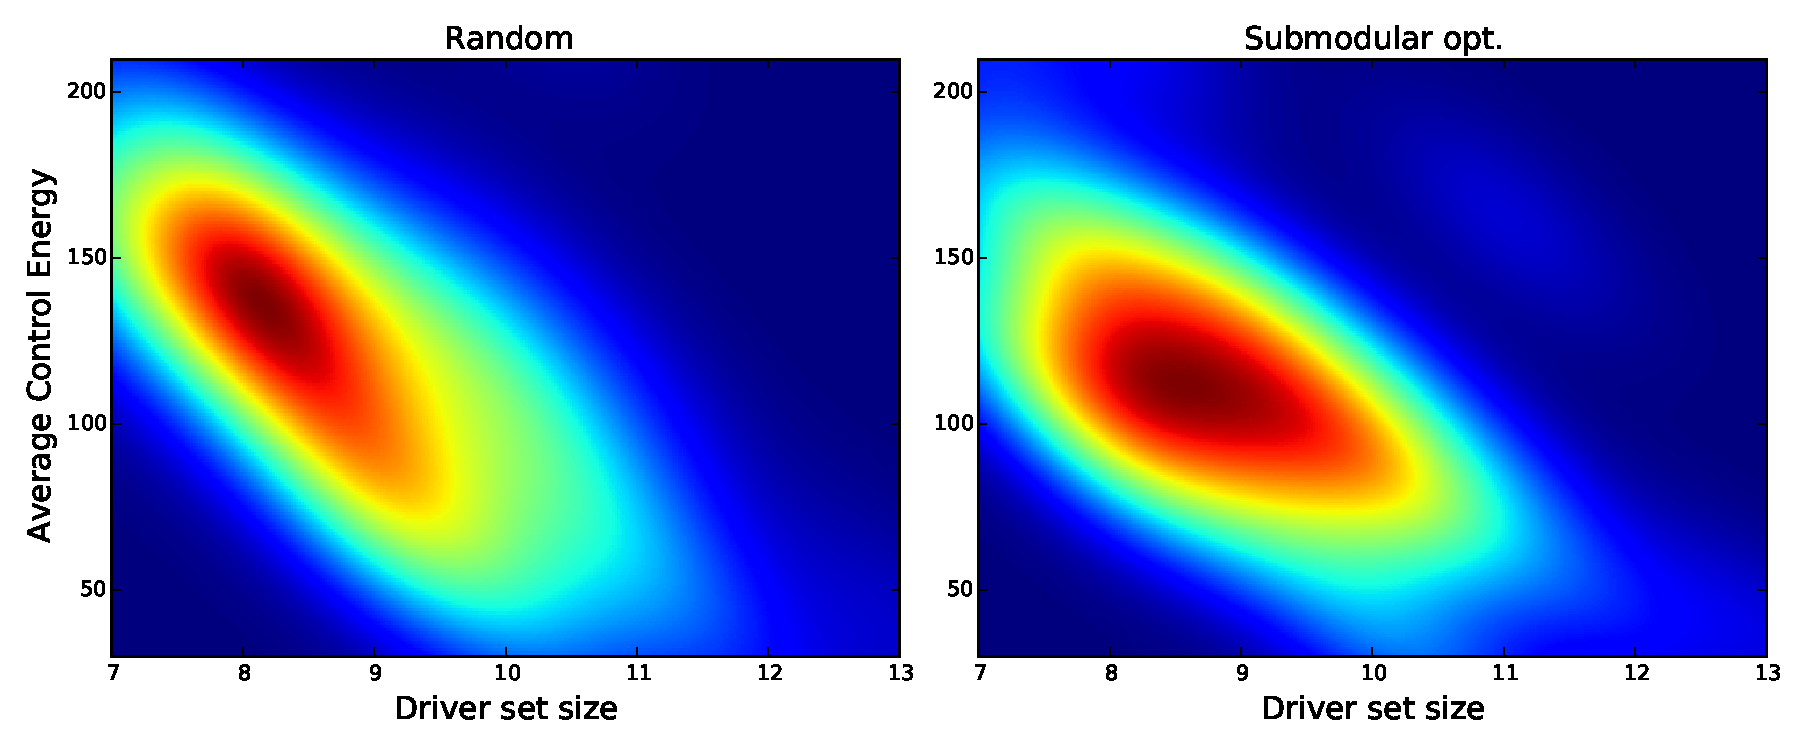
\includegraphics[scale=.35]{rr.pdf}
	\end{figure}
\end{frame}



\end{document}
